%
% Academic CV LaTeX (filled with content from PersonalResume.docx)
% Template Author: Dubasi Pavan Kumar (MIT)
% Filled for: Yinghui He
%

\documentclass[a4paper,11pt]{article}

% Package imports
\usepackage{latexsym}
\usepackage{xcolor}
\usepackage{float}
\usepackage{ragged2e}
\usepackage[empty]{fullpage}
\usepackage{wrapfig}
\usepackage{tabularx}
\usepackage{titlesec}
\usepackage{geometry}
\usepackage{marvosym}
\usepackage{verbatim}
\usepackage{enumitem}
\usepackage{fancyhdr}
\usepackage{multicol}
\usepackage{graphicx}
\usepackage{cfr-lm}
\usepackage[T1]{fontenc}
\usepackage{fontawesome5}
\usepackage{academicons}
\usepackage{tikz}
\usepackage[absolute,overlay]{textpos}


% Color definitions
% \definecolor{darkblue}{rgb}{0, 0, 0.5}
\definecolor{darkblue}{HTML}{1D63A6}
\definecolor{darkred}{HTML}{A6231D}

% Page layout
\setlength{\multicolsep}{0pt} 
\pagestyle{fancy}
\fancyhf{} % clear all header and footer fields
\fancyfoot{}
\renewcommand{\headrulewidth}{0pt}
\renewcommand{\footrulewidth}{0pt}
\geometry{left=1.4cm, top=0.8cm, right=1.2cm, bottom=1cm}
\setlength{\footskip}{5pt}

% Hyperlink setup
\usepackage[hidelinks]{hyperref}
\hypersetup{
    colorlinks=true,
    linkcolor=darkblue,
    filecolor=darkblue,
    urlcolor=darkblue,
}

% Custom box settings
\usepackage[most]{tcolorbox}
\tcbset{
    frame code={},
    center title,
    left=0pt,
    right=0pt,
    top=0pt,
    bottom=0pt,
    colback=gray!20,
    colframe=white,
    width=\dimexpr\textwidth\relax,
    enlarge left by=-2mm,
    boxsep=4pt,
    arc=0pt,outer arc=0pt,
}

% URL style
\urlstyle{same}

% Text alignment
\raggedright
\setlength{\tabcolsep}{0in}

% Section formatting
\titleformat{\section}{
  \vspace{-4pt}\scshape\raggedright\large
}{}{0em}{}[\color{black}\titlerule \vspace{-7pt}]

% Custom commands
\newcommand{\resumeItem}[2]{
  \item{
    \textbf{#1}{\hspace{0.5mm}#2 \vspace{-0.5mm}}
  }
}
\newcommand{\resumePOR}[3]{
\vspace{0.5mm}\item
    \begin{tabular*}{0.97\textwidth}[t]{l@{\extracolsep{\fill}}r}
        \textbf{#1}\hspace{0.3mm}#2 & \textit{\small{#3}} 
    \end{tabular*}
    \vspace{-2mm}
}
\newcommand{\resumeSubheading}[4]{
\vspace{0.5mm}\item
    \begin{tabular*}{0.98\textwidth}[t]{l@{\extracolsep{\fill}}r}
        \textbf{#1} & \textit{\footnotesize{#4}} \\
        \textit{\footnotesize{#3}} &  \footnotesize{#2}\\
    \end{tabular*}
    \vspace{-2.4mm}
}

\newcommand{\resumePublication}[4]{
\vspace{0.5mm}
    \begin{tabular*}{0.98\textwidth}[t]{@{}p{0.66\textwidth} @{\extracolsep{\fill}} >{\raggedleft\arraybackslash}p{0.30\textwidth}@{}}
        \textbf{#1} & \textbf{\footnotesize{#4}} \\
        #3 &  \textit{\footnotesize{#2}}\\
    \end{tabular*}\\[-0.4em]
}


\newcommand{\resumeProject}[4]{
\vspace{0.5mm}\item
    \begin{tabular*}{0.98\textwidth}[t]{l@{\extracolsep{\fill}}r}
        \textbf{#1} & \textit{\footnotesize{#3}} \\
        \footnotesize{\textit{#2}} & \footnotesize{#4}
    \end{tabular*}
    \vspace{-2.4mm}
}
\newcommand{\resumeSubItem}[2]{\resumeItem{#1}{#2}\vspace{-4pt}}

\renewcommand{\labelitemi}{$\vcenter{\hbox{\tiny$\bullet$}}$}
\renewcommand{\labelitemii}{$\vcenter{\hbox{\tiny$\circ$}}$}

\newcommand{\resumeSubHeadingListStart}{\begin{itemize}[leftmargin=*,labelsep=1mm]}
\newcommand{\resumeHeadingSkillStart}{\begin{itemize}[leftmargin=*,itemsep=1.7mm, rightmargin=2ex]}
\newcommand{\resumeItemListStart}{\begin{itemize}[leftmargin=*,labelsep=1mm,itemsep=0.5mm]}
\newcommand{\resumeSubHeadingListEnd}{\end{itemize}\vspace{2mm}}
\newcommand{\resumeHeadingSkillEnd}{\end{itemize}\vspace{-2mm}}
\newcommand{\resumeItemListEnd}{\end{itemize}\vspace{-2mm}}
\newcommand{\cvsection}[1]{%
\vspace{2mm}
\begin{tcolorbox}
    \textbf{\large #1}
\end{tcolorbox}
    \vspace{-4mm}
}

\newcolumntype{L}{>{\raggedright\arraybackslash}X}%
\newcolumntype{R}{>{\raggedleft\arraybackslash}X}%
\newcolumntype{C}{>{\centering\arraybackslash}X}%

% Font options
\newcommand{\headerfonti}{\fontfamily{phv}\selectfont} % Helvetica-like (similar to Arial/Calibri)
\newcommand{\headerfontii}{\fontfamily{ptm}\selectfont} % Times-like (similar to Times New Roman)
\newcommand{\headerfontiii}{\fontfamily{ppl}\selectfont} % Palatino (elegant serif)
\newcommand{\headerfontiv}{\fontfamily{pbk}\selectfont} % Bookman (readable serif)
\newcommand{\headerfontv}{\fontfamily{pag}\selectfont} % Avant Garde-like (similar to Trebuchet MS)
\newcommand{\headerfontvi}{\fontfamily{cmss}\selectfont} % Computer Modern Sans Serif
\newcommand{\headerfontvii}{\fontfamily{qhv}\selectfont} % Quasi-Helvetica (another Arial/Calibri alternative)
\newcommand{\headerfontviii}{\fontfamily{qpl}\selectfont} % Quasi-Palatino (another elegant serif option)
\newcommand{\headerfontix}{\fontfamily{qtm}\selectfont} % Quasi-Times (another Times New Roman alternative)
\newcommand{\headerfontx}{\fontfamily{bch}\selectfont} % Charter (clean serif font)


% Commands for icon sizing and positioning
\newcommand{\socialicon}[1]{\raisebox{-0.05em}{\resizebox{!}{1em}{#1}}}
\newcommand{\ieeeicon}[1]{\raisebox{-0.3em}{\resizebox{!}{1.3em}{#1}}}

\pagestyle{fancy}
\fancyhf{} % clear default
% \fancyfoot[C]{\thepage} % page number centered at footer

\begin{document}
\headerfontiii

%-------------------- Header --------------------%
% \begin{center}
%     {\Huge\textbf{Yinghui He}}
% \end{center}
% \vspace{-6mm}

% \begin{center}
%     \small{
%     % +1-734-834-7390 | 
%     \href{mailto:yh0068@princeton.edu}{yh0068@princeton.edu} | 
%     \href{https://ying-hui-he.github.io}{Website}
%     } |
%     \href{https://scholar.google.com/citations?user=HGVRBCoAAAAJ&hl=en}{Google Scholar} |
%     \href{https://www.linkedin.com/in/yinghui-he-300238346/}{\socialicon{\faLinkedin}}
%     \href{https://github.com/ying-hui-he}{\socialicon{\faGithub} }
%     % \ieeeicon{
\includegraphics[height=1.3em]{ieee_collabratec_icon.png}} \href{https://ieee-collabratec.ieee.org/app/p/your-profile}{your-profile} |
%     \href{https://x.com/yinghui_he_}{\socialicon{\faTwitter}}
% \end{center}
% \vspace{-6mm}

% --- Header ---
\noindent
\begin{minipage}[t]{0.74\textwidth}
\vspace{0pt} % top-align with the photo
{\Huge\textbf{Yinghui He}}\par
\vspace{2pt}
{\small
\href{mailto:yh0068@princeton.edu}{yh0068@princeton.edu} \,|\, 
\href{https://ying-hui-he.github.io}{Website} \,|\, 
\href{https://scholar.google.com/citations?user=HGVRBCoAAAAJ&hl=en}{Google Scholar} \,|\, 
\href{https://www.linkedin.com/in/yinghui-he/}{\socialicon{\faLinkedin}}\,
\href{https://github.com/ying-hui-he}{\socialicon{\faGithub}}\,
\href{https://x.com/yinghui_he_}{\socialicon{\faTwitter}}
}
\end{minipage}%
\hfill
\begin{minipage}[t]{0.22\textwidth}
\vspace{0pt}
\raggedleft
% Replace 'photo.jpg' and adjust size as needed
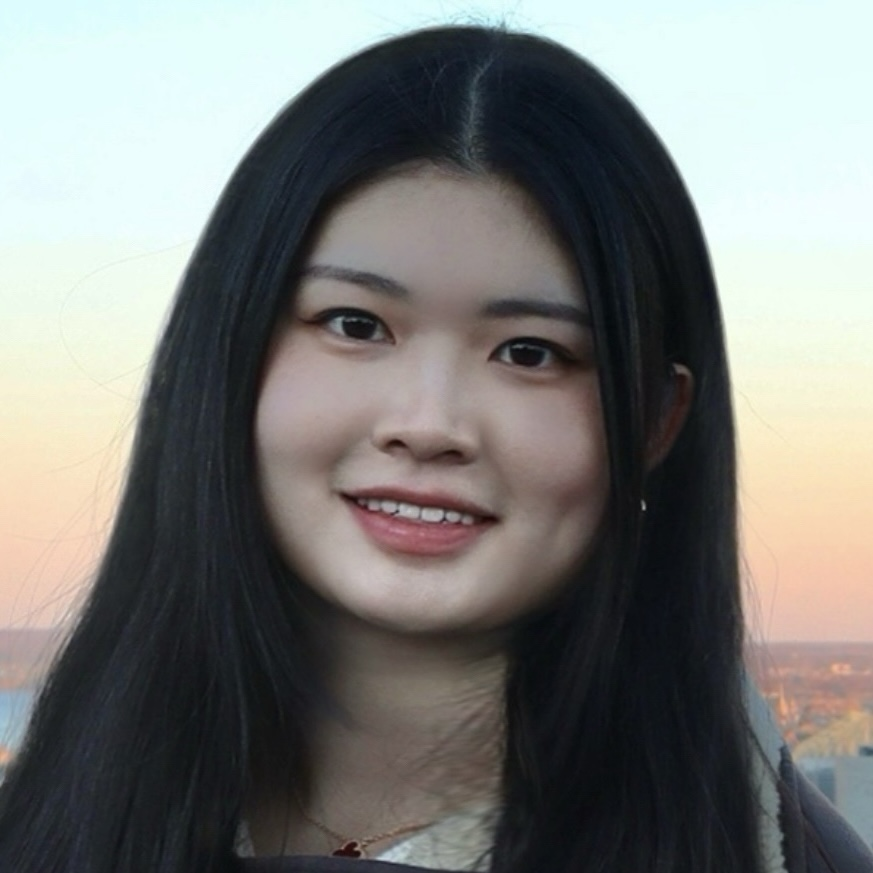
\includegraphics[width=0.8in,height=0.8in,keepaspectratio]{profile2_large.jpg}
\end{minipage}
% --- End Header ---
\vspace{-5mm}


%-------------------- Education --------------------%
\section{\textbf{Education}}
\vspace{-0.4mm}

\normalsize{
\resumeSubHeadingListStart

\resumeSubheading
{Princeton University}{Princeton, NJ}
{Ph.D. Candidate in Computer Science. Advised by \href{https://www.cs.princeton.edu/~arora/}{Sanjeev Arora}.}{September 2024 -- June 2029 (Anticipated)}

\resumeSubheading
{University of Michigan}{Ann Arbor, MI}
{B.S.E. in Computer Science \& B.S. (Minor) in Mathematics. (GPA: 3.98 / 4.00)}{September 2022 -- May 2024}
% \resumeItemListStart
%   \item GPA: 3.981 / 4.00
% \resumeItemListEnd

\resumeSubheading
{Shanghai Jiao Tong University}{Shanghai, China}
{B.E. in Electrical and Computer Engineering. (GPA: 3.93 / 4.00; Ranking: 1 / 221)}{September 2022 -- August 2024}
% \resumeItemListStart
%   \item GPA: 3.929 / 4.00; Ranking: 1 / 221
% \resumeItemListEnd

\resumeSubHeadingListEnd
}

\vspace{-6mm}

%-------------------- Publications --------------------%
\section{\textbf{Projects \& Publications}}
\vspace{0.2mm}
\small{
% \resumePublication
% {\textbf{Skill-Targeted Adaptive Training}}{Princeton University}{\textbf{Yinghui He$^*$}, Abhishek Panigrahi$^*$, Yong Lin, Sanjeev Arora.}{(Under Review)}
% \begin{itemize}[leftmargin=*, itemsep=0.2mm]
%   \item Introduced AdaptMI, an adaptive method to select skill-based in-context examples that boosts performance by 6\%.
%   \item 
% \end{itemize}
\vspace{0.5mm}
% Row 1: title (narrow, wraps) + workshops (right-aligned via nested tabular)
\begin{tabular*}{0.98\textwidth}[t]{@{}p{0.52\textwidth} @{\extracolsep{\fill}} >{\raggedleft\arraybackslash}p{0.41\textwidth}@{}}
    \href{https://arxiv.org/abs/2604.12002}{\textbf{Self-Distillation Zero: Self-Revision Turns Binary Rewards into Dense Supervision}} &
    \begin{tabular}[t]{@{}r@{}}
        \textbf{\footnotesize{ICML 2026 RLxF Workshop \textcolor{darkred}{\textbf{(Oral)}};}} \\
        \textbf{\footnotesize{AI4Math Workshop \textcolor{darkred}{\textbf{(Honorable Mention)}}}}
    \end{tabular} \\
\end{tabular*}\\[0em]
% Row 2: authors (wide) + university (right-aligned, single line)
\begin{tabular*}{0.98\textwidth}[t]{@{}p{0.78\textwidth} @{\extracolsep{\fill}}r@{}}
    \textbf{Yinghui He}, , Simran Kaur, Adithya Bhaskar, Yongjin Yang, Jiarui Liu, Narutatsu Ri, Liam Fowl, Abhishek Panigrahi, Danqi Chen, and Sanjeev Arora. & \textit{\footnotesize{Princeton University}}\\
\end{tabular*}\\[-0.4em]
\begin{itemize}[leftmargin=*, itemsep=0.2mm]
  \item Proposed SD-Zero, an on-policy self-distillation method that converts binary rewards into dense token supervision.
    \item Conducted experiments on Qwen3 and Olmo3 models across math and code benchmarks and brought $10\%$ gains.
    % outperforming strong baselines including RFT, GRPO, and SDFT under the same training sample budget.
\end{itemize}

\resumePublication
{\href{https://arxiv.org/abs/2510.10023}{\textbf{Skill-Targeted Adaptive Training
}}}{Princeton University}{\textbf{Yinghui He*}, Abhishek Panigrahi*, Yong Lin, and Sanjeev Arora.}{ICLR 2026}
\begin{itemize}[leftmargin=*, itemsep=0.2mm]
  \item Proposed STAT, an adaptive training strategy that constructs training data targeted at models' missing skills.
  \item Solely implemented data creation pipeline; conducted SFT and RL training on Llama and Qwen models.
\end{itemize}

\resumePublication
{\href{https://arxiv.org/abs/2505.00147}{\textbf{AdaptMI: Adaptive Skill-based In-context Math Instruction for Small Language Models}}}{Princeton University}{\textbf{Yinghui He}, Abhishek Panigrahi, Yong Lin, and Sanjeev Arora.}{COLM 2025}

\begin{itemize}[leftmargin=*, itemsep=0.2mm]
  \item Introduced AdaptMI, an adaptive method that boosts in-context performance by 6\% through skill-based examples.
  \item Solely conducted experiments on Llama and Qwen models (1B--7B), and large-scale skill labeling with GPT-4o.
\end{itemize}


\resumePublication
{\href{https://arxiv.org/abs/2310.16755}{\textbf{Hi-ToM: A Benchmark for Evaluating Higher-Order Theory of Mind Reasoning in LLMs}}}{University of Michigan}{
\textbf{Yinghui He}, Yufan Wu, Yilin Jia, Rada Mihalcea, Yulong Chen, and Naihao Deng.}{EMNLP 2023}

\begin{itemize}[leftmargin=*, itemsep=0.2mm]
  \item Released the Hi-ToM benchmark that tests the higher-order theory of mind abilities in LLMs \href{https://scholar.google.com/citations?view_op=view_citation&hl=en&user=HGVRBCoAAAAJ&citation_for_view=HGVRBCoAAAAJ:u5HHmVD_uO8C}{(cited by 100+)}.
  \item Independently implemented an automated data generator; coordinated human annotation on 600+ samples.
\end{itemize}

\resumePublication
{\href{https://arxiv.org/abs/2504.09689}{\textbf{EmoAgent: Assessing and Safeguarding Human-AI Interaction for Mental Health Safety}}}{Princeton University}{Jiahao Qiu*, \textbf{Yinghui He}*, Xinzhe Juan, Yimin Wang, Yuhan Liu, Zixin Yao, Yue Wu, Xun Jiang, Ling Yang, and Mengdi Wang.}{EMNLP 2025}

\begin{itemize}[leftmargin=*, itemsep=0.2mm]
  \item Built EmoAgent, a multi-agent AI framework to mitigate mental health risks by over 50\% in human–AI interactions.
  % \item Found 57.6\% of interactions led to mental state deterioration; proposed EmoGuard reduced risks by over 50\%.
  \item Co-led experimental design and result analysis; coordinated the EmoAgent team.
\end{itemize}

\resumePublication
{\href{https://arxiv.org/abs/2504.09689}{\textbf{Making Complex Reasoning Student-Friendly: A Hybrid Distillation Framework}}}{Princeton University}{Yongjin Yang, \textbf{Yinghui He}, Jiarui Liu, and Zhijing Jin.}{Under Submission (2026)}

\begin{itemize}[leftmargin=*, itemsep=0.2mm]
  \item Proposed SFD, a hybrid distillation method that switches from teacher to student using entropy/NLL-based gating.
  \item Implemented dynamic student rewrite to reduce distribution shift, applying to 6 reasoning benchmarks.  
\end{itemize}

\resumePublication
{\href{https://arxiv.org/abs/2501.05414}{\textbf{LongProc: Benchmarking Long-Context Language Models on Long Procedural Generation}}}{Princeton University}{Xi Ye, Fangcong Yin*, \textbf{Yinghui He}*, Joie Zhang*, Howard Yen*, Tianyu Gao, Greg Durrett, and Danqi Chen.}{COLM 2025}

\begin{itemize}[leftmargin=*, itemsep=0.2mm]
    \item Introduced LongProc, a benchmark that tests both long-form generation and highly dispersed information.

  % \item Built a theory-of-mind tracking task within LongProc for evaluating LCLMs on long-form procedural generation.
  \item Independently designed and generated 2k examples for the \textit{Theory-of-Mind Tracking} subset, and evaluated 17 LLMs.
\end{itemize}
}
\vspace{-6mm}

%-------------------- Internship Experience --------------------%
\section{\textbf{Internship}}
\vspace{-0.4mm}
\resumeSubHeadingListStart
\resumeSubheading
{NVIDIA}{Santa Clara, CA}
{Research Scientist Intern}{May 2026 -- August 2026} \vspace{2mm}
\resumeItemListStart
    \item Involved in the development of NVIDIA Nemotron models.
  \item Studied algorithms \& data curation for on-policy distillation on multi-turn agentic settings.
\resumeItemListEnd

\resumeSubheading
{VMware}{Shanghai, China}
{Research Intern}{July 2022 -- October 2022} \vspace{2mm}
\resumeItemListStart
  % \item Reviewed literature on federated analytics; identified unexplored areas.
  \item Studied algorithms and applications of federated analytics; proposed optimization methods on federated analytics.
\resumeItemListEnd

\resumeSubHeadingListEnd
\vspace{-7mm}

%-------------------- Scholarships --------------------%
\section{\textbf{Scholarships}}
\vspace{-0.4mm}
\resumeSubHeadingListStart

\resumePOR{Chinese National Scholarship}{, Ministry of Education of the People’s Republic of China}{\textyen{}8000 (\$1170)}
\resumeItemListStart
  \item Highest scholarship in China awarded to Top 1\% college students.
\resumeItemListEnd

\resumePOR{Fan Xuji Scholarship}{, Shanghai Jiao Tong University}{\textyen{}20000 (\$2940)}
\resumeItemListStart
  \item Highest SJTU scholarship awarded to 18 all-round developed students.
\resumeItemListEnd

\resumePOR{SJTU Undergraduate Excellence Scholarship}{, Shanghai Jiao Tong University}{\textyen{}1000 (\$150)}
\resumeItemListStart
  \item Awarded to top-ranking (10\%) students.
\resumeItemListEnd

\resumePOR{John Wu and Jane Sun Excellence Scholarship}{, UM-SJTU Joint Institute}{\textyen{}75000 (\$11000)}
\resumeItemListStart
  \item Highest scholarship in UM-SJTU Joint Institute awarded to 10 all-round developed students.
\resumeItemListEnd

\resumePOR{The Jackson and Muriel Lum Scholarship}{, UM-SJTU Joint Institute}{\$14000}
\resumeItemListStart
  \item Awarded to 5 excellent students in the dual-degree program.
\resumeItemListEnd

\resumeSubHeadingListEnd
\vspace{-6mm}

%-------------------- Skills --------------------%
\section{\textbf{Technical Skills}}
\vspace{-0.4mm}
 \resumeHeadingSkillStart
  \resumeSubItem{Programming Languages: }
    {Python, C++, C, C\#, Java, JavaScript, HTML/CSS, SQL}
    \resumeSubItem{Model Training: }
    {Multi-node \& distributed training, Verl, TRL (Transformers Reinforcement Learning), LoRA, DeepSpeed, PyTorch, TensorFlow, scikit-learn, NumPy, pandas}
  \resumeSubItem{Model Inference: }
    {vLLM, Hugging Face Transformers, Accelerate, quantization \& efficient serving}
  \resumeSubItem{Agentic Frameworks: }
    {LangChain, AutoGen, Hugging Face Hub, APIs}
  \resumeSubItem{Data Science \& Mathematical Tools: }
    {pandas, NumPy, Matplotlib, Seaborn, SciPy, Jupyter, Colab, MATLAB, R, Mathematica, SymPy}
 \resumeHeadingSkillEnd


%-------------------- Honors & Awards --------------------%
\section{\textbf{Honors and Awards}}
\vspace{-0.4mm}
\resumeSubHeadingListStart

\resumeProject
  {Dean’s List}
  {Outstanding GPA, University of Michigan}
  {2023, 2024}
  {}

\resumeProject
  {Mathematical Contest in Modelling}
  {Consortium for Mathematics and its Applications}
  {Finalist Award (2\%), May 2022}
  {}

\resumeProject
  {University Physics Competition}
  {UPC Committee}
  {Bronze Medal, December 2021}
  {}

\resumeProject
  {Media University-Enterprise Global Innovation Competition}
  {Media Shanghai}
  {First Place, November 2021}
  {}

\resumeProject
  {United Nations Global Youth Leadership Academy Summer Learning Program}
  {GYLA}
  {Outstanding Participant, August 2021}
  {}

\resumeSubHeadingListEnd
% \vspace{-6mm}

%-------------------- Teaching Experience --------------------%
\section{\textbf{Teaching \& Advising}}
\vspace{-0.4mm}
\resumeSubHeadingListStart

\resumeSubheading
{Teaching Assistant}{Shanghai Jiao Tong University}
{Physics II (60 students), Chemistry I (150 students)}{September 2021 -- August 2022}

\resumeSubheading
{Student Advisor}{Shanghai Jiao Tong University}
{UM-SJTU Joint Institute Advising Center}{September 2021 -- August 2022}

\resumeSubheading
{Writing Consultant}{Shanghai Jiao Tong University}
{UM-SJTU Joint Institute Writing Center}{September 2021 -- August 2023}

\resumeSubHeadingListEnd
% \vspace{-6mm}

%-------------------- Society Membership & Extracurricular --------------------%
\section{\textbf{Extracurricular Activities}}
\vspace{-0.4mm}
\resumeSubHeadingListStart

\resumePOR{Society of Women Engineers (SWE)}{, Member}{}

\resumePOR{Princeton Koko Pops Dance Company}{, Member}{}

\resumePOR{UMich Heartbeat A Cappella Group}{, Song Arranger, Soprano}{}

\resumePOR{UMich Moli Dance Group}{, Member}{}

\resumeSubHeadingListEnd

% (Sections like Objective, Projects, Skills, Volunteer Experience, Professional Memberships (beyond SWE),
% Certifications, Additional Information, References are intentionally omitted to mirror the original DOCX content.)

\end{document}